\documentclass{sigchi}

% Use this section to set the ACM copyright statement (e.g. for
% preprints).  Consult the conference website for the camera-ready
% copyright statement.

% Copyright
\CopyrightYear{2016}
%\setcopyright{acmcopyright}
\setcopyright{acmlicensed}
%\setcopyright{rightsretained}
%\setcopyright{usgov}
%\setcopyright{usgovmixed}
%\setcopyright{cagov}
%\setcopyright{cagovmixed}
% DOI
\doi{http://dx.doi.org/10.475/123_4}
% ISBN
\isbn{123-4567-24-567/08/06}
%Conference
\conferenceinfo{CHI'16,}{May 07--12, 2016, San Jose, CA, USA}
%Price
\acmPrice{\$15.00}

% Use this command to override the default ACM copyright statement
% (e.g. for preprints).  Consult the conference website for the
% camera-ready copyright statement.


%% HOW TO OVERRIDE THE DEFAULT COPYRIGHT STRIP --
%% Please note you need to make sure the copy for your specific
%% license is used here!
% \toappear{
% Permission to make digital or hard copies of all or part of this work
% for personal or classroom use is granted without fee provided that
% copies are not made or distributed for profit or commercial advantage
% and that copies bear this notice and the full citation on the first
% page. Copyrights for components of this work owned by others than ACM
% must be honored. Abstracting with credit is permitted. To copy
% otherwise, or republish, to post on servers or to redistribute to
% lists, requires prior specific permission and/or a fee. Request
% permissions from \href{mailto:Permissions@acm.org}{Permissions@acm.org}. \\
% \emph{CHI '16},  May 07--12, 2016, San Jose, CA, USA \\
% ACM xxx-x-xxxx-xxxx-x/xx/xx\ldots \$15.00 \\
% DOI: \url{http://dx.doi.org/xx.xxxx/xxxxxxx.xxxxxxx}
% }

% Arabic page numbers for submission.  Remove this line to eliminate
% page numbers for the camera ready copy
% \pagenumbering{arabic}

% Load basic packages
\usepackage{balance}       % to better equalize the last page
\usepackage{graphics}      % for EPS, load graphicx instead 
\usepackage[T1]{fontenc}   % for umlauts and other diaeresis
\usepackage{txfonts}
\usepackage{mathptmx}
\usepackage[pdflang={en-US},pdftex]{hyperref}
\usepackage{color}
\usepackage{booktabs}
\usepackage{textcomp}

% Some optional stuff you might like/need.
\usepackage{microtype}        % Improved Tracking and Kerning
% \usepackage[all]{hypcap}    % Fixes bug in hyperref caption linking
\usepackage{ccicons}          % Cite your images correctly!
% \usepackage[utf8]{inputenc} % for a UTF8 editor only
\usepackage{float}

% If you want to use todo notes, marginpars etc. during creation of
% your draft document, you have to enable the "chi_draft" option for
% the document class. To do this, change the very first line to:
% "\documentclass[chi_draft]{sigchi}". You can then place todo notes
% by using the "\todo{...}"  command. Make sure to disable the draft
% option again before submitting your final document.
\usepackage{todonotes}

% Paper metadata (use plain text, for PDF inclusion and later
% re-using, if desired).  Use \emtpyauthor when submitting for review
% so you remain anonymous.
\def\plaintitle{}
\def\plainauthor{First Author, Second Author, Third Author,
  Fourth Author, Fifth Author, Sixth Author}
\def\emptyauthor{}
\def\plainkeywords{Authors' choice; of terms; separated; by
  semicolons; include commas, within terms only; required.}
\def\plaingeneralterms{Documentation, Standardization}

% llt: Define a global style for URLs, rather that the default one
\makeatletter
\def\url@leostyle{%
  \@ifundefined{selectfont}{
    \def\UrlFont{\sf}
  }{
    \def\UrlFont{\small\bf\ttfamily}
  }}
\makeatother
\urlstyle{leo}

% To make various LaTeX processors do the right thing with page size.
\def\pprw{8.5in}
\def\pprh{11in}
\special{papersize=\pprw,\pprh}
\setlength{\paperwidth}{\pprw}
\setlength{\paperheight}{\pprh}
\setlength{\pdfpagewidth}{\pprw}
\setlength{\pdfpageheight}{\pprh}

% Make sure hyperref comes last of your loaded packages, to give it a
% fighting chance of not being over-written, since its job is to
% redefine many LaTeX commands.
\definecolor{linkColor}{RGB}{6,125,233}
\hypersetup{%
  pdftitle={\plaintitle},
% Use \plainauthor for final version.
%  pdfauthor={\plainauthor},
  pdfauthor={\emptyauthor},
  pdfkeywords={\plainkeywords},
  pdfdisplaydoctitle=true, % For Accessibility
  bookmarksnumbered,
  pdfstartview={FitH},
  colorlinks,
  citecolor=black,
  filecolor=black,
  linkcolor=black,
  urlcolor=linkColor,
  breaklinks=true,
  hypertexnames=false
}

% create a shortcut to typeset table headings
% \newcommand\tabhead[1]{\small\textbf{#1}}

% End of preamble. Here it comes the document.
\begin{document}

\title{Milestone 1\\ Discovering Unaligned Expectations in Universities and Industry for New Graduates in Computer Science and Software Engineering and Finding Possible Solutions}

\numberofauthors{2}
\author{%
  \alignauthor{Alan Franzoni\\
    \affaddr{Georgia Institute of Technology}\\
    \affaddr{Trieste, Italy}\\
    \email{alan.franzoni@gatech.edu}}\\
  \alignauthor{Hasti Ghabel\\
    \affaddr{Georgia Institute of Technology}\\
    \affaddr{Atlanta, GA}\\
    \email{hghabel1@gatech.edu}}\\
}

\maketitle

\section{About our research}
We focus on discovering whether there is a misalignment in university and industry expectations for new graduates. We are considering four groups including: 1-undergraduate students, 2-post-graduate students,3- professors, teachers, or university staff, and 4-industry professionals. In our final project, we will also collect the data on what would be some possible solutions to reduce the skill gap, which is caused by expectation gap among these four groups.

\textit{\textbf{Our Research Questions}}\newline
We will direct two sets of questions in our final project. In the first set, our main question is: \textbf{does the perceived skill gap in fresh graduates exist because the academy is unable to provide a good training, or just because a) the academy is not even trying to do that kind of job, and b) the industry is taking that kind of job for granted, or c) the students think they should be getting something that the university has no intention to provide them with?} Here, we ask what could be the reasons that there exist a gap between students, professors, and industry professionals' expectations. We will look into these questions for both \textbf{undergraduate} and \textbf{post-graduate} level students that are recently graduated from school. We also ask the question that \textbf{how the students' degree can improve the chance of getting hired? Do the graduate-level studies help the students to gain adaptive skills in industry more quickly?}\newline
In the second set of our questions, we are asking \textbf{what would be the best solutions that bring the university and industry's objectives closer to each other?} 


\textit{\textbf{Our Hypothesis}}\newline
\textit{Hypothesis 1}: One of the reasons for the perceived skill gap is that all those that should - in an employer's view - care for learning some skills to be used at work, don't actually have that aim during their education phase. In other words, the misaligned expectations between industry and university causes the skill gap. Those skills have impact on job proficiency and possibilities to get hired. We think that the expectations among four groups differ. These four groups are composed of \textbf{undergraduate-level students, post-graduate-level students, educators and school staff, and industry professionals}. The main problem is not only that one side hasn’t enough resources or skills to achieve a certain goal, but, rather, that there’s a different vision or gaol on what should be done, and different and unaligned \textit{rewards} exist for different groups.  

\textit{Hypothesis 2}:  We think that the following hypothesis is that the graduate-level studies, on the contrary, can play an important role on reducing the skill gap between industry and university, and therefore, can be considered as one good resolution for that issue. More specifically, we think that \textbf{high-quality online graduate-level programs} such as Georgia Tech OMSCS (Online Master of Science in Computer Science) are quite aligned with industry expectations. These such programs also target many people from all over the world, who can become proficient in their job quickly as well as being active in an academic environment.

\section{review research methodologies}
During this milestone, we focused on three of our sample groups: "undergraduate students", "professors, teachers, and university staff", "industry professionals". We provided three sets of surveys; one for each group. The surveys were written in GoogleFoms. Below, you can find the link to the survey for each group:\\

\textbf{Student (undergraduate level) group}:\\ \textcolor{blue}{https://goo.gl/forms/G4s5dtDZL9chZ1zt1}\\

\textbf{Professors, Teachers, and University Staff group}: \\ \textcolor{blue}{https://goo.gl/forms/jg20dElqkg1oCNiI2}\\

\textbf{Industry Professionals group}:\\  \textcolor{blue}{https://goo.gl/forms/4UCemOlDdaScKz952}\\

We shared the survey links with our classmates on PeerSurvey website (http://peersurvey.cc.gatech.edu/). We used our classmates as a small sample of participants. In order to recruit as many participants as possible, we created a thread in Piazza, where we described our research goals and asked our classmates to take our survey if they are interested. We asked them to submit the survey for one group category that matches the best with their current position. 

In our surveys, we provided one last open-ended question about their thoughts regarding the quality and quantity of the survey questions; Is there any questions that could be asked that we missed adding it in our survey? Is there any misunderstanding in any of the questions that could be described better for the participants? Here our goal was to receive feedback from participants and understand how we can improve the survey questions before sending it to the other general audience. We discuss about the feedbacks in the later sections of this paper.

\section{Demo of the Website}
In order to send our survey to the general audience, we planned to create a website, where we can write about our goals and describe the research. During this milestone, we set-up the website and put the content there. Our website can be found under link: \textcolor{blue}{http://www.misalignedtech.com/}
We will also add our finalized survey link there. This section will be completed after the survey becomes ready. In the end, we are planning to share the result we find on the website for whoever interested to see the results. We are planning to share the website on social media (Facebook, LinkedIn, etc.), OMCS slack channels, Piazza and anywhere that we can recruit enough participants.

We created a short demo of our website. Please use the link below to view the demo of our website:

\url{https://youtu.be/hXOf_RYrcPA}


\section{Results}
We were able to collect total of 54 responses from all three categories. The break down for each category: Student survey = 28 responses, Professor, Teachers, and University Staff survey = 3 responses, and Industry Professionals survey = 23 responses.
We will go through the results for each of the categories separately.

\textit{\textbf{STUDENTS}}\newline
The age of most of the participants in this category was 27 year old. Around 92\% of the participants live in the US and 8\% from other countries, which split into France and China.  Above 80\% of the participants' major (at undergraduate-level) was in computer science or any similar technology related fields. Some other, around 17\%, were coming from other fields such as business and marketing. Among those, 64\% of participants' latest degree is BS, around 28\% have already their masters, and around 7\% have PHD. We found that most of the students received their degree form the US, but we also had other countries including China, India, and France.

We looked into the students' goals of studying computer science. We received about 75\% of the responses toward the reason that they are interested in this field (figure 1).

\begin{figure}
\centering
  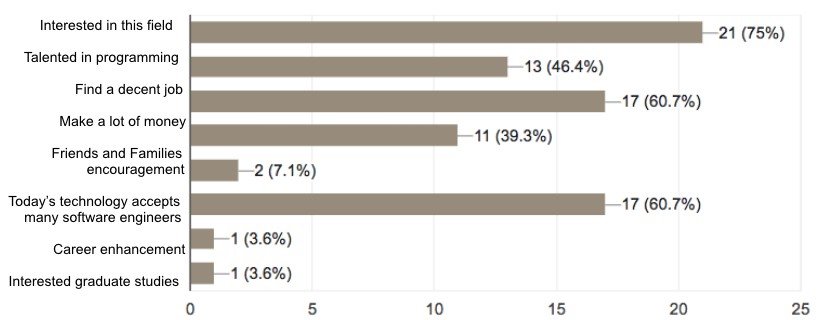
\includegraphics[width=1.05\columnwidth]{figures/goals_s}
  \caption{The student responses to the survey question: What are the current goals of studying computer science in undergraduate level? }~\label{fig:figure1}
\end{figure}

In the next level, we are interested to see what are the ideal goals of studying computer science. About 64\% of the participants' ideal goal was to learn about computer science and its fundamentals. Interestingly, the second high selected answer, about 57\%, was to get into industry very quickly (figure 2).

\begin{figure}
\centering
  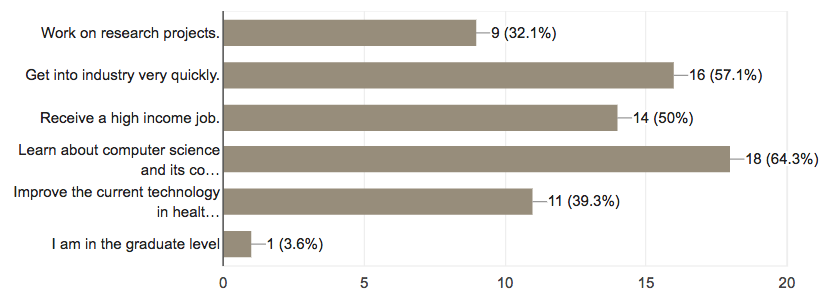
\includegraphics[width=1.05\columnwidth]{figures/ideal_goals_s}
  \caption{The student responses to the survey question: In your opinion, what are the ideal goals of studying computer science in undergraduate level?}~\label{fig:figure2}
\end{figure}

We looked at some factors that can play a role in finding a job for new graduates. Some of those factors are GPA, university that the student graduates from, or gaining the skills from a university compared to learning it from any available online courses. We created a rating questions which had the response options of "very important", "important", "neutral", "not important", and "not at all". The result for each of the questions are shown in a table in figure 3. As it shows, many students think that all three factors play an important role in finding a job when they graduate from school.

The participants mostly believed that having a university degree is important to land a job. Per the responses, some of the reasons are as:
\begin{itemize}
	\item Receiving a degree says that you have learned fundamentals, worked with others on a team, have adequate written and verbal communication skills.
	\item It is very easy to give up in the middle in an online setting.
	\item Getting technical jobs, the recruiters heavily reaches out to graduate students of top institutions vs smaller schools due to the fact of prestige and rigor of work.
	\item Many companies still filter out candidates who don't have a degree. While you can self-teach yourself many concepts, a degree curriculum can make you more well-rounded.
\end{itemize}

On the other hand there were responses that described the university degree is not very important in getting hired. Some examples are shown below:
\begin{itemize}
	\item With online MOOCs it's giving everyone an opportunity to understand the concepts of CS. Degree is no longer important.
	\item A degree from an accredited university does not mean anything. Any company claiming to be a "school" can be nationally "accredited". Search online for the term "diploma mills"
	\item To land a job, you need to have a specific skill set and be able to use certain tools and platforms in line with the companies products. College does not teach this but companies such as Udacity Nanodegree / bootcamps are backed by the actual companies that you want to work for.
\end{itemize}


\begin{figure}
\centering
  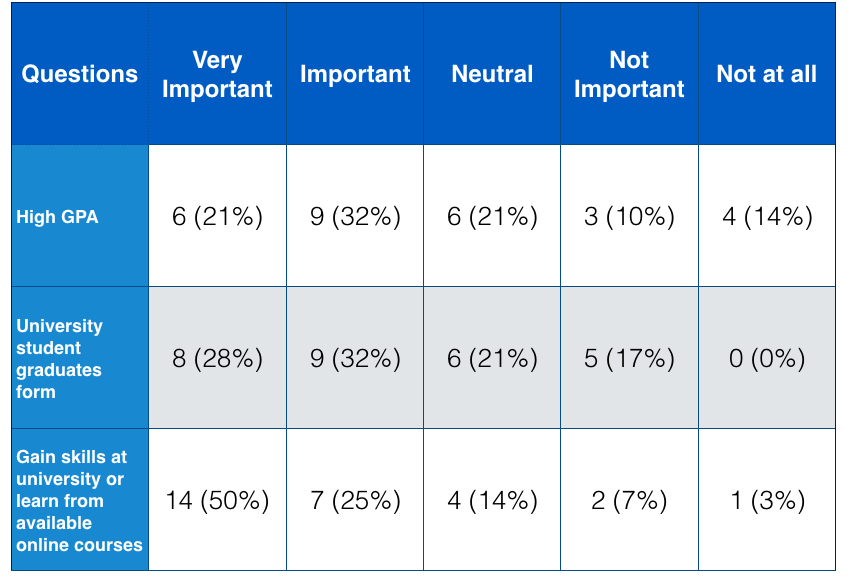
\includegraphics[width=1.05\columnwidth]{figures/important_notimportant_table_s}
  \caption{The student rated each questions and selected one of the response options from "very important", "important", "neutral", "not important", and "not at all". Each row shows the item that can play a role in finding a job for new graduates. The columns are the response options}~\label{fig:figure3}
\end{figure}

Many students (39\%) think that there would be a transition time between 1-3 months for a new graduate to get hired. 17\% of the students mentioned that the undergraduate student already have a job in a computer science related field (figure 4).

\begin{figure}
\centering
  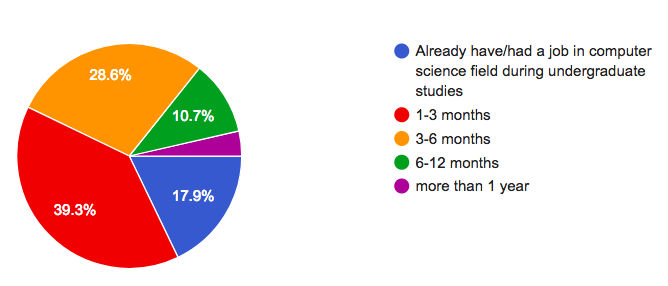
\includegraphics[width=1.05\columnwidth]{figures/transition_time_s}
  \caption{The student responses to the survey question: For an undergraduate-level student, what would be the transition time from graduation to start the first job? }~\label{fig:figure4}
\end{figure}

We also looked in the the time required for a new graduate to become proficient in their future or current job. Interestingly, the response options get very similar percentages. Each of the options of "3-6 months" and "6-12 months" received 25\% of the responses. About 28\% of students think that the new graduates become proficient in their job in 1-3 months and 21\% of students think that proficiency in job takes more than 1 year (figure 5).

\begin{figure}
\centering
  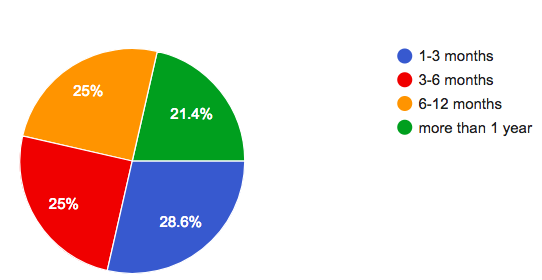
\includegraphics[width=1.05\columnwidth]{figures/time_proficiency_s}
  \caption{The student responses to the survey question: What would be the required time for a new graduate to become proficient in their current/future job? }~\label{fig:figure5}
\end{figure}


\textit{\textbf{INDUSTRY PROFESSIONALS}}\newline
We had the age range from 22 to 55 years old. Participants with the age of 26 and 34 years old had the highest percentage of participantion (13\%).
Same as student group, around 92\% of the participants live in the US and 8\% from other countries, which split into Colombia and India. Among the participants, 94\% of participants' latest degree is BS, and around 6\% have already their master's degree. The average size of the organization division is about 600 people. 

Per industry professionals, the current goal of universities on teaching computer science is to teach undergraduate students the theoretical topics in this field (78\%). The other main selected goal was to be teach analytical thinking skills (16\%). Only 10\% of the industry professionals believe that the goal of universities for undergraduate studies is to prepare students for their future job. 
We also asked that what would be the \textbf{ideal} goal of undergraduate studies to become successful in future job. The industry professionals believe that the ideal university goal should be teaching structures of computer science (69\%) and preparing students to get into industry very quickly (65\%).

We asked the same questions regarding the importance of GPA, university the student graduates, and gaining skills from degree studies, from industry professionals as well. The result is shown in the table in figure 6.
The participants mostly believed that having a university degree is important to land a job. Per the responses, some of the reasons are as:
\begin{itemize}
	\item Universities usually teaches at higher standards.
	\item Having a degree from accredited university puts the candidate ahead of other crowd so that could be considered as an advantage.
	\item Candidates without university degree just don't know the fundamentals and do not have the four years of university taught critical thinking skills.
	\item Universities usually have critical thinking components that most certifications lack, university education involves a deep understanding of computing systems, usually university eduction involves some form of project based courses where students have to produce original works rather than follow a specific curriculum.
\end{itemize}
On the other side, there were some ideas that university degree is not very important and gaining the skills from any other resources is enough to land a job. One of the interesting response was described as "Some (even prestigious) universities don't teach all that well, and even worse, don't grade effectively. It is very possible for students to get a degree without learning much beyond first year level. Conversely, with the amount of resources available online, a motivated individual can learn much more than is covered in a university degree. Most BS degrees waste a lot of time on classes outside the major and even classes within the major often aren't strenuous enough."
 
\begin{figure}
\centering
  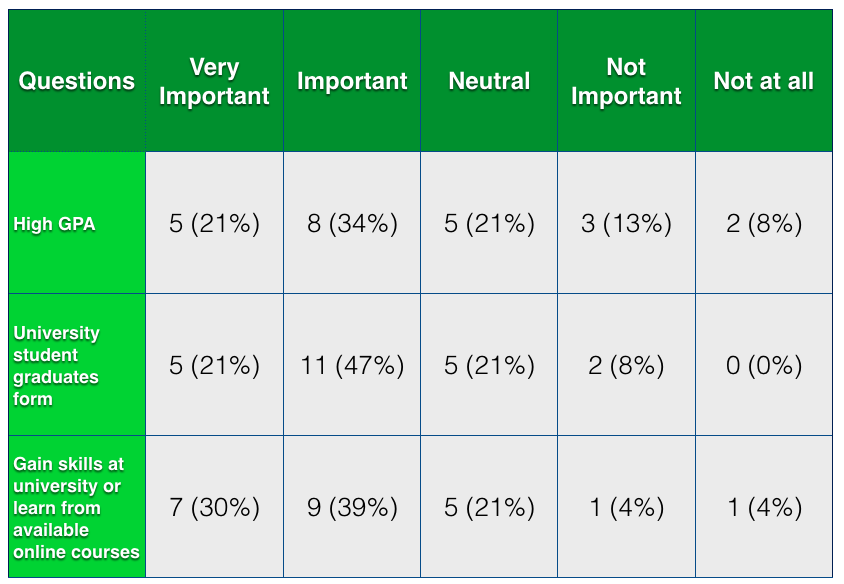
\includegraphics[width=1.05\columnwidth]{figures/important_notimportant_table_i}
  \caption{The industry professionals rated each questions and selected one of the response options from "very important", "important", "neutral", "not important", and "not at all". Each row shows the item that can play a role in finding a job for new graduates. The columns are the response options}~\label{fig:figure6}
\end{figure}

Most of industry professionals think that there would be 1-3 months time transition for new graduates in computer science to find a new job (34\%). We received the same amount of responses (34\%) that the undergraduate students work in a company during their studies (figure 7).

\begin{figure}
\centering
  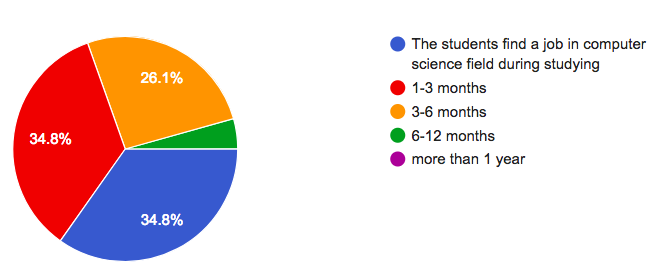
\includegraphics[width=1.05\columnwidth]{figures/transition_time_i}
  \caption{The industry professionals responses to the survey question: For an undergraduate-level student, what would be the transition time from graduation to start the first job? }~\label{fig:figure7}
\end{figure}

Interestingly, contrary to students' opinions, industry professionals think that it takes about 1 year for a new graduate to become proficient in their future/current job (35\%). Only 4\% thinks that it will take 1-3 months to become proficient in the job (figure 8).

\begin{figure}
\centering
  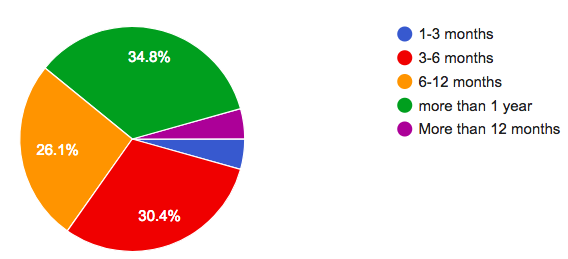
\includegraphics[width=1.05\columnwidth]{figures/time_proficiency_i}
  \caption{The industry professionals responses to the survey question: What would be the required time for a new graduate to become proficient in their current/future job? *correction on the figure: the option of "more than 1 year: was exchanged with "more than 12 months" option.}~\label{fig:figure8}
\end{figure}

\textit{\textbf{PROFESSORS, TEACHERS, UNIVERSITY STAFF}}\newline
We did not receive a good amount of responses for this category. Only 3 people attended in this category. We cannot provide the results confidently. But one interesting point is about current goal and ideal goal of academic environment on teaching computer science to undergraduate students. Their votes for current goal is to "teach programming languages" and the ideal goal was that students should "work on research topics in computer science fields". This point is very interesting, since it is very different from industry professionals' and also students' opinions.

\begin{figure}
\centering
  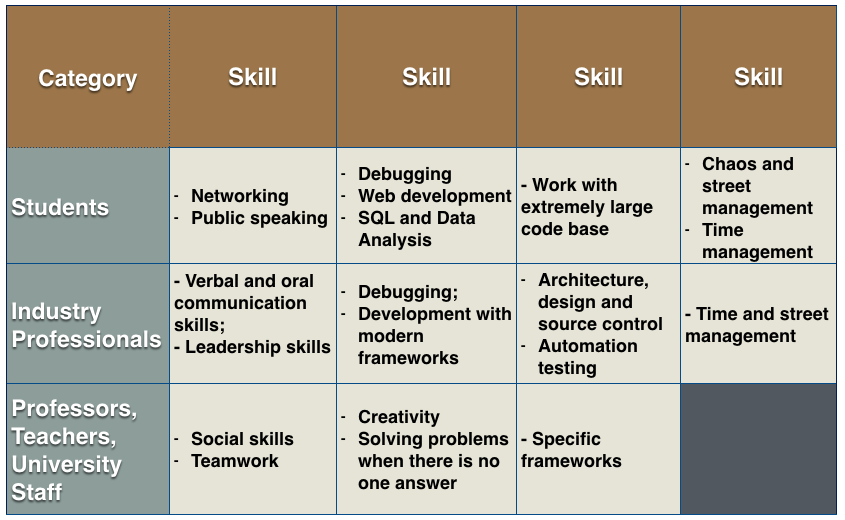
\includegraphics[width=1.05\columnwidth]{figures/skills}
  \caption{Summary of responses for all three categories to the question: What are the top skills that are useful and important for a job that might not be taught in schools or universities, if any? Please specify 2-3 items. (Use N/A if not applicable)}~\label{fig:figure9}
\end{figure}


\section{Survey Feedback}
Most of the participants gave us good comments and they liked our short survey questionnaire. We also received some productive feedback, which we will consider them in our next step. We collected some of the feedbacks and listed them below:
\begin{itemize}
	\item "I think that the survey was fine, I think it may help to understand what kind of school the survey respondent to? That could affect the results."
	\item "I think this survey did a great job covering the topic. I am interested to see the results."
	\item "It wasn't always clear if I was supposed to be answering from *purely* my perspective disregarding societal expectations. For example when answering "in my opinion having a high GPA [answer]" -- I personally don't care at all about GPA, but I acknowledge that many many other people do and therefore that means it ought to be a consideration. In some of your later questions you asked "why did you answer the way you did", which I think would be good to have for all like scale questions."
	\item "I don't like open-ended questions because they take longer to complete on a mobile phone."
	\item "spellcheck and ensure the student can answer the questions truthfully, leave options like "Other" and keep each question to one single question."
	\item "I think demographic information would be pertinent as well. I don't think you can put a general blanket over everyone (i.e. men vs. women might have differing ideas)"
	\item "It was a great survey, no issues"
	\item "Looks comprehensive as it is"
\end{itemize}


\section{Progress Report}
During this milestone, we were able to create the first draft of our survey and share it with our classmates. We've got total of 54 participants for all the categories. We asked from ourself how good is our survey and how the questions can help us to move toward our hypothesis. As we collected and analyzed this data sample, we learnt about the problems of some of the question types. 
We received many feedbacks from the participants, which helped us to improve our survey questions. We applied many of the feedbacks and planed a new set of questions for the general audience survey. 

Some of our other achievements were setting up our website and testing it to make sure it opens in different browsers. We also decided to use R programming for our data analysis.

 \section{Future Steps}
In our next step, we are planning to create one single survey and put a single questions in the beginning of the survey that the participants can select their category. We will make it multiple selection option, since one participant can be a student as well as an industry professional.

We will have two types of questions in our survey. One would be multiple choice questions and the second part is open-ended questions. The first part focuses on discovery the misaligned expectations between undergraduate students, post-graduate students, professors, teachers or university staff, and industry professionals. The second part is a qualitative survey and will focus on finding the solutions to reduce the skill gap in industry for new graduates. We need to collect the responses to the open-ended questions as soon as we receive any data. The qualitative analysis will be a little time consuming and needs to review and analyze all the answers.

Our plan is to refresh our knowledge in R programming and data analysis. We will use R programming tool to analyze the data and then, collect the results.

\section{Updated survey}

After collecting some feedback, we turned the survey into just one, and added some questions to distinguish between graduate and undergraduate level. You can see a draft of our work, which will go live shortly, here:

\url{https://www.dropbox.com/s/ktz6geuinh3ty3e/First_Draft_Survey_Questions.pdf?dl=0}
 

\balance{}

\balance{}

% REFERENCES FORMAT
% References must be the same font size as other body text.
%\bibliographystyle{SIGCHI-Reference-Format}
%\bibliography{../bibliography.bib}

\end{document}

%%% Local Variables:
%%% mode: latex
%%% TeX-master: t
%%% End:
 